\documentclass[a4paper,10pt,titlepage,bibtotoc,bibtotocnumbered]{scrreprt}

\usepackage[utf8]{inputenc}
\usepackage[pdftex]{graphicx}
\usepackage{lscape}
\usepackage{rotating}
\usepackage{ulem}


%%%%%%%Here you have to choose german or english texts in your submissions
%German submission
%\usepackage[ngerman]{babel}
%English submission
\usepackage[english]{babel}

%Graphics and pictures
\usepackage[caption=false]{subfig}
\usepackage{float}
\restylefloat{figure}
\usepackage{placeins}

%Enumerations
\usepackage{enumerate}
\usepackage{mdwlist}

%Math symbols
\usepackage{amsmath}
\usepackage{amssymb}

%Coloring of tables
\usepackage{longtable}
\usepackage{xcolor, colortbl}

%Code representation
\usepackage{listings}

%Diagrams with tikZ
\usepackage{tikz}
\usetikzlibrary{shapes.geometric, arrows, positioning}

\newcommand{\students}[1]{\def\vstudents{#1}}
\newcommand{\labtime}[1]{\def\vlabtime{#1}}
\newcommand{\supervisor}[2]{\def\vsupervisor{\href{#2}{#1}}}


\usepackage[marginpar=2cm,
	reversemp,
	includehead,
	includefoot,
	bindingoffset=0cm,
	textheight=23cm,
	hdivide={3.5cm,*,3.5cm},
	vdivide={*,23cm,*}
	]{geometry}


\usepackage[pdftex,	pdfauthor={},
				pdftitle={Cinema Management Application},
				pdfsubject={Lab for Software Engineering WS22/23}, 
				breaklinks=true, 
				colorlinks=true, 
				linkcolor=black,
				urlcolor=blue,%blue
				citecolor=red,%red
	        		pdfpagemode=None,
%   			    	pdffitwindow=true,
        			a4paper=true,
				plainpages=false,
				pdfpagelabels,     
				pageanchor=false,
				pdfstartpage=1,
           ]{hyperref}


\begin{document} 


%-------------------- Declaration part --------------------------------------------
%-------------------- Here you have to add all group members, your lab date -------
%-------------------- and the name of your supervisor -----------------------------
\students{Ifrat Jahan (3098878)\\Jennifer Maxisch (3106694)\\Georgios Adamos (3093306)\\Thomas Klimek (3067855)\\Melvin van der Linde (3106762)}
\labtime{Do. 12-14}
\supervisor{Marcel Schweikert}{marcel.schweikert@stud.uni-due.de} % email unconfirmed
%----------------------------------------------------------------------------------
%----------------------------------------------------------------------------------



\pagenumbering{roman}

\begin{titlepage}
\centering
\enlargethispage*{40mm}

\vspace*{-10mm}

\begin{minipage}[c]{0.25\textwidth}
\hspace*{-22mm}

\includegraphics[height=45pt]{figures/logo_uni}\linebreak
\end{minipage}
\begin{minipage}[r]{0.74\textwidth}
\vspace*{1mm}
\begin{flushright}
\Large{Lab for Software Engineering}\linebreak
\large{Winter term 2022/2023}\linebreak
\end{flushright}
\end{minipage}
\hspace*{-18mm}

\textcolor{blue}{\rule{154mm}{0.2mm}}


\vspace*{55mm}\vfill

\textit{Lab for Software Engineering}\vspace*{4mm}

\Huge{Cinema Management Application}\vspace*{7mm}

\Large{\vstudents}\vspace*{9mm}


\normalsize{\today}



\vspace*{80mm}

\textcolor{blue}{\rule{\textwidth}{0.2mm}}
\begin{flushleft}
\sf University of Duisburg-Essen $\cdot$ Faculty of Engineering
\large{Working group \href{http://swe.uni-due.de}{Software Engineering} -- Prof. Dr. M. Heisel}\\

\small{Date: \vlabtime- Supervisor: \vsupervisor}
\end{flushleft}

\end{titlepage}


\tableofcontents
\listoffigures

%------------
%------------The structure is the same as used in the lecture.
%------------You can specify new sections included in each chapter and you can also add new subsections.
%------------
%------------
\chapter{Analysis}
\section{A1}

%---------------
%---------------The style of enumerations is already given (e.g. R1, R2,...)
%---------------Just add \item before each element
%---------------
%---------------
\subsection{Requirements \& Domain-Knowledge}

\subsubsection{Requirements}
\begin{enumerate}[R1]
	\item Customers can create an account by providing an e-mail address and a password. If an e-mail address which is already associated with an account is provided, account creation fails.
    \item Customers can log in by providing their e-mail address and their password.
    \item A logged in customer can log out.
    \item A customer can browse available showings, ascendingly sorted by date.
    \item A logged in customer can book tickets by selecting the showing from the browsing list and selecting the desired seats. A showing can only be booked up to 15 minutes before it starts.
    \item Staff can add new showings to the database by providing the required data.
    \item Once a showing starts it is marked as "archived".
    \item Archived showings are visible to staff, but not to customers.
    \item Staff can cancel showings. When a show is cancelled all customers who booked tickets for it are notified via e-mail and the showing is then deleted.
    \item Showings which took place a year ago or longer are automatically removed from the database.
    \item When a showing is deleted its associated bookings are also deleted.
    
\end{enumerate}

\subsubsection{Facts}
\begin{enumerate}[F1]
	\item A showing consists of the title of the movie, its duration, the date date, the hall number and unique ID.
	\item A hall consists of a number of rows, a number of seats per row and a unique hall number.
    \item Only one person at a time can sit in a seat.
\end{enumerate}

\subsubsection{Assumptions}
\begin{enumerate}[{A}1]
	\item A web application is a good choice for implementing the desired functionality and all customers are able to use it.
	\item Customers only provide e-mail addresses they can access.
    \item Customers will stay up to date with the list of available showings.
    \item Every booking is paid via an external service.
    \item Staff will only add showings which take place in the future.
\end{enumerate}

%---------------
%---------------You can use the following code snippet to inclue pictures into your document.
%---------------\caption command places a little description under the picture.
%---------------\label is used to reference the picture in the text with command \ref{figure:contextDiagram}.
%---------------
\subsection{Contextdiagram}
\begin{figure}[H]
	\centering
  	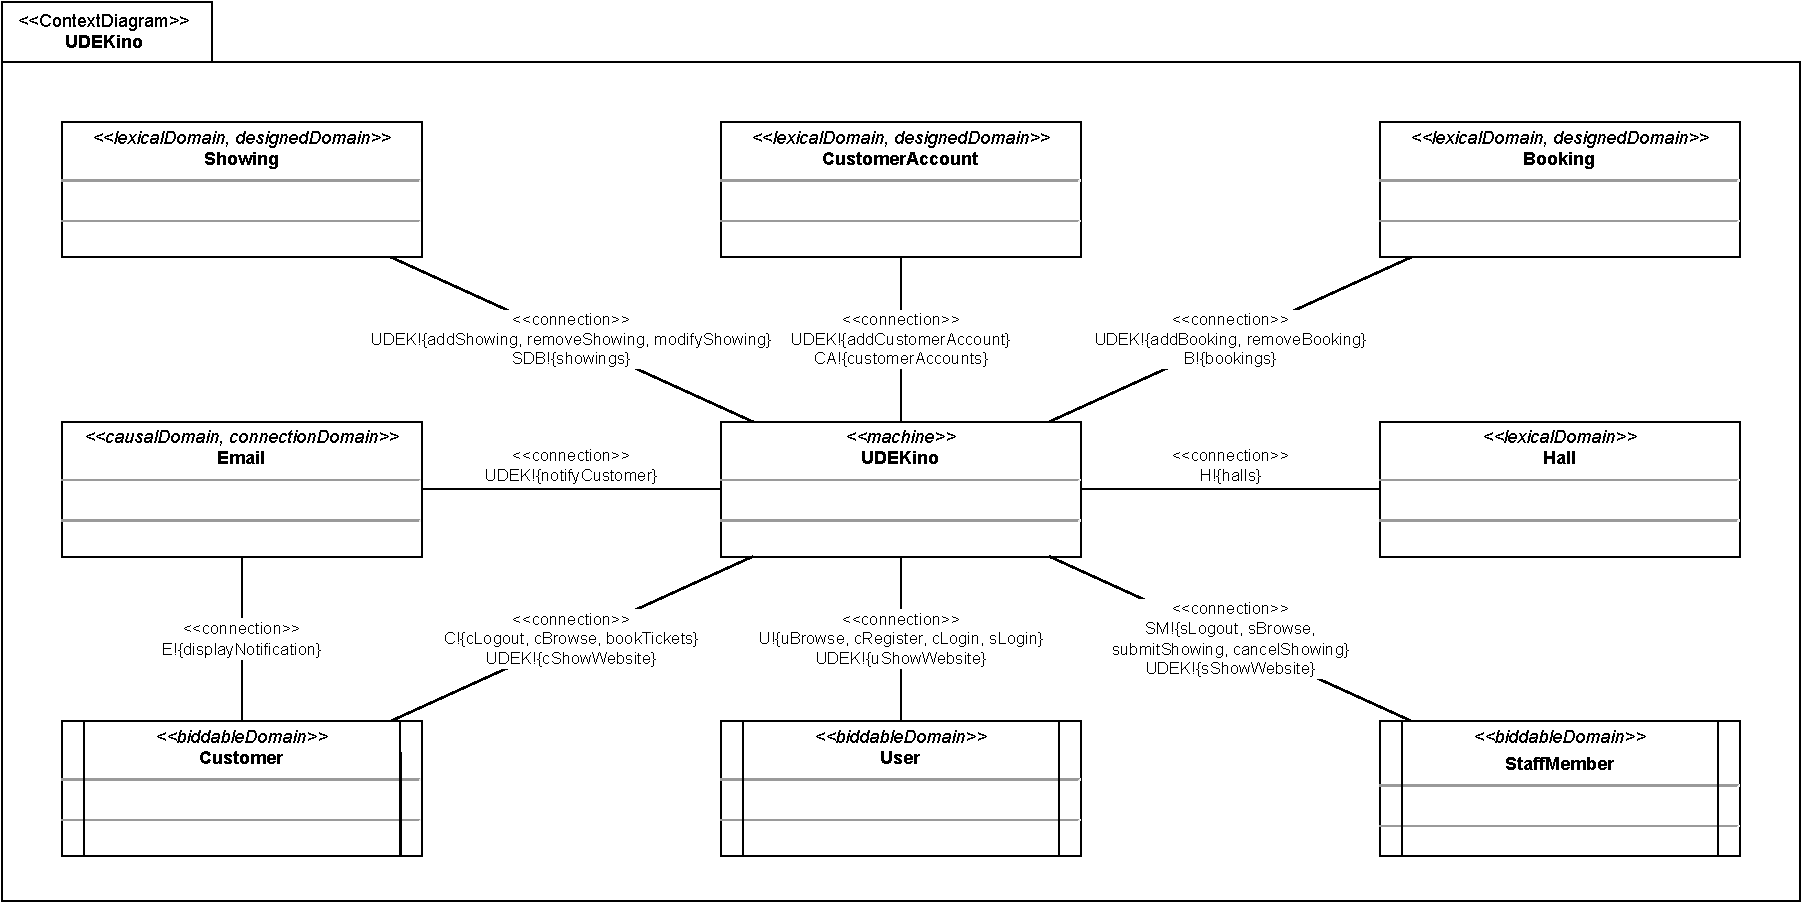
\includegraphics[width=0.9\textwidth]{figures/02/a02_context_diagram.pdf}
	\caption{Contextdiagram}
	\label{figure:contextDiagram}
\end{figure}


\newpage\section{A2}
We can derive the following problem diagrams

\begin{figure}[H]
	\centering
  	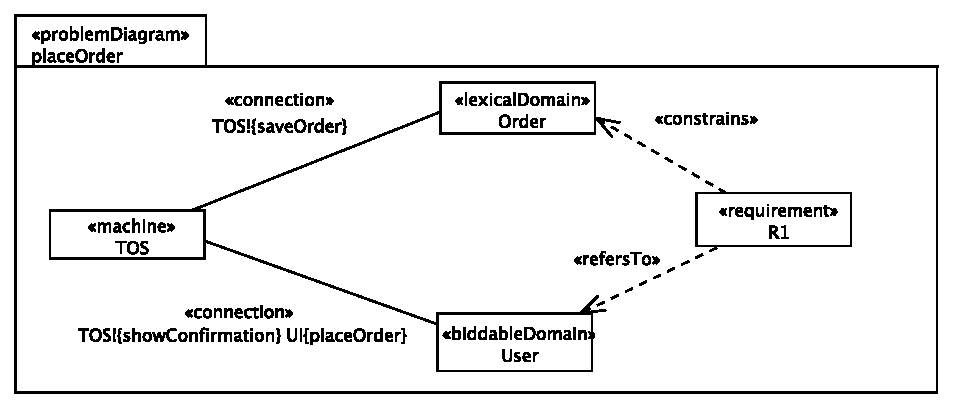
\includegraphics[width=0.9\textwidth]{figures/A2/pdR1.pdf}
	\caption{Problemdiagram for R1}
	\label{figure:pdR1}
\end{figure}

\newpage\section{A3}

\newpage\section{A4}

\newpage\section{A5}
A short OCL example:\\
%-------------------
%-------------------The following used package provides an easy OCL syntax highlighting.
%-------------------You do not have to add linebreaks. It is done automatically.
%-------------------
\lstset{language=OCL}          % Set your language (you can change the language for each code-block optionally)

\begin{lstlisting}[frame=single,breaklines=true,numbers=left,numberfirstline=true]
context Person inv: self.alter >=0

pre alter>30
post alter=alter@pre+1

\end{lstlisting}

\newpage\section{A6}

Examples of a life-cycle using the math-environment:

$LC_{guest}=(Browse^+;[Book])^*$



\chapter{Design}

\section{D1}

\section{D2}

\section{D3}

\section{D4}

State diagrams with tikZ:
%Do not change, only declaration of the element
\tikzstyle{startpoint} = [circle, minimum width=0.5cm, minimum height=0.5cm, text centered, draw=black, fill=black]
\tikzstyle{endpoint} = [circle, minimum width=0.5cm, minimum height=0.5cm, text centered, draw=black, fill=white]
\tikzstyle{endin} = [circle, minimum width=0.05cm, minimum height=0.05cm, text centered, draw=black, fill=black]
\tikzstyle{state} = [rectangle, rounded corners, minimum width=2cm, minimum height=1cm, text centered, draw=black]
\tikzstyle{decision} = [diamond, minimum width=0.5cm, minimum height=0.5cm, text centered, draw=black]
\tikzstyle{arrow} = [->,>=stealth]
\tikzstyle{every node} = [font=\tiny]

%--------------
%--------------We use the same figure environment as for pictures to reference diagrams with tikz.
%--------------Here we provide a small example how to draw a state machine with tikZ.
%--------------The picture is created only with this commands.
%--------------
\begin{figure}[H]
\caption{Zustandsdiagramm Person 1}
\label{d1:zustand1}
\begin{tikzpicture}[node distance=2cm]

%Knoten
\node (Start) [startpoint]{};
\node (State1) [state, right= of Start] {State 1};
\draw [arrow] (Start) -- (State1);

\node (Decision1) [decision, right= of State1]{};
\draw [arrow] (State1) -- (Decision1)  node [pos=0.5,below,fill=white] {Annotation};

\node (State2) [state, below= of Decision1] {State 2};
\draw [arrow] (Decision1) -- (State2)  node [pos=0.2,below,fill=white] {true};



\node (End) [endpoint,right= of State2]{\begin{tikzpicture}\node (End) [endin]{};\end{tikzpicture}};
\draw [arrow] (State2) -- (End);
\draw [arrow] (Decision1) -| (End)  node [pos=0.2,left,fill=white] {false};
\end{tikzpicture}
\end{figure}



\chapter{Implementation \& Testing}

%---------------
%---------------You do not have to copy your source code.
%---------------Just use the given space to add any comments or explanations.
%---------------

\section{I}

\section{T1}

\section{T2}

\section{T3}




%-------------------------
%-------------------------
%--------The glossary makes use of the package longtable to allow automatic page breaks
%-------------------------
%-------------------------
\chapter{Glossary}

\begin{longtable}{|l|l|p{5cm}|l|}
\caption{Glossary} 
\label{table:glossar}\\ 
\hline
\rowcolor{black!25}\textbf{Name} & \textbf{Type} & \textbf{Description} & \textbf{Source}\\
\hline
\endfirsthead
\caption[]{Glossar}\\ 
\hline
\rowcolor{black!25}\textbf{Name} & \textbf{Type} & \textbf{Description} & \textbf{Source}\\
\endhead
\hline
\endfoot
\multicolumn{4}{|l|}{\textbf{A}}\\
\hline
%-------------------------
%-------------------------
%--------Each element of the table is expressed in the following way:
%--------Cells are divided by & and each row ends with \\ (linebreak).
%--------The line between two rows is added with \hline.
%-------------------------
%-------------------------
addBooking & phenomenom & the machine adds a booking to the BookingsDatabase & CD\\
\hline
addCustomer & phenomenon & the machinea adds a customer to the CustomersDatabase & CD\\
\hline
addShowings & phenomenon & the machine adds a showing to the ShowingsDatabase & CD\\
\hline
addStaffMember & phenomenon & the machine adds a staff account to the StaffDatabase & CD\\
\hline
%-------------------------
%-------------------------
\multicolumn{4}{|l|}{\textbf{B}}\\
\hline
BookingsDatabase & lexical domain, designed domain & the database of bookings made by customers & CD\\
\hline
\multicolumn{4}{|l|}{\textbf{C}}\\
\hline
Customer & biddable domain & a customer of UDEKino & CD\\
\hline
CustomersDatabase & lexical domain, designed domain & the database of Customer accounts & CD\\
\hline
cBook & phenomenon & a customer books tickets for a showing & CD\\
\hline
cBrowse & phenomenon & a customer browses available showings & CD\\
\hline
cLogin & phenomenon & a customer attempts to log in & CD\\
\hline
cLogout & phenomenon & a customer attempts to log out & CD\\
\hline
cRegister & phenomenon & a customer attempts to register create an account on UDEKino & CD\\
\hline
cShowWebsite & phenomenon & the machine shows a website to the Customer & CD\\
\hline
\multicolumn{4}{|l|}{\textbf{D}}\\
\hline
&  &  & \\
\hline
\multicolumn{4}{|l|}{\textbf{E}}\\
\hline
Email & causal domain, connection domain & an e-mail service offering to deliver e-mails & CD\\
\hline
\multicolumn{4}{|l|}{\textbf{F}}\\
\hline
&  &  & \\
\hline
\multicolumn{4}{|l|}{\textbf{G}}\\
\hline
&  &  & \\
\hline
\multicolumn{4}{|l|}{\textbf{H}}\\
\hline
&  &  & \\
\hline
\multicolumn{4}{|l|}{\textbf{I}}\\
\hline
&  &  & \\
\hline
\multicolumn{4}{|l|}{\textbf{J}}\\
\hline
&  &  & \\
\hline
\multicolumn{4}{|l|}{\textbf{K}}\\
\hline
&  &  & \\
\hline
\multicolumn{4}{|l|}{\textbf{L}}\\
\hline
LoggedInCustomer & biddable domain & a customer who has logged into their account & CD\\
\hline
lcShowWebsite & phenomenon & the machine shows a website to the LoggedInCustomer & CD\\
\multicolumn{4}{|l|}{\textbf{M}}\\
\hline
modifyShowing & phenomenon & the machine modifies a showing in the database & CD\\
\hline
\multicolumn{4}{|l|}{\textbf{N}}\\
\hline
notifyCustomer & phenomenon & the machine notifies the customer via e-mail & CD\\
\hline
\multicolumn{4}{|l|}{\textbf{O}}\\
\hline
&  &  & \\
\hline
\multicolumn{4}{|l|}{\textbf{P}}\\
\hline
&  &  & \\
\hline
\multicolumn{4}{|l|}{\textbf{Q}}\\
\hline
&  &  & \\
\hline
\multicolumn{4}{|l|}{\textbf{R}}\\
\hline
&  &  & \\
\hline
\multicolumn{4}{|l|}{\textbf{S}}\\
\hline
sAddShowing & phenomenon & a staff member submits a new showing to the machine for entry into the database & CD\\
\hline
sBrowse & phenomenon & a staff member browses available showings & CD\\
\hline
sCancelShowing & phenomenon & a staff member attempts to cancel a showing & CD\\
\hline
ShowingsDatabase & lexical domain, designed domain & the database of Showings & CD\\
\hline
sShowWebsite & phenomenon & the machine shows a website to the StaffMember & CD\\
\hline
StaffDatabase & lexical domain, designed domain & the database of Staff accounts & CD\\
\hline
StaffMember & biddable domain & a member of UDEKino staff & CD\\
\hline
\multicolumn{4}{|l|}{\textbf{T}}\\
\hline
&  &  & \\
\hline
\multicolumn{4}{|l|}{\textbf{U}}\\
\hline
&  &  & \\
\hline
\multicolumn{4}{|l|}{\textbf{V}}\\
\hline
%&  &  & \\
\hline
\multicolumn{4}{|l|}{\textbf{W}}\\
\hline
&  &  & \\
\hline
\multicolumn{4}{|l|}{\textbf{X}}\\
\hline
&  &  & \\
\hline
\multicolumn{4}{|l|}{\textbf{Y}}\\
\hline
yieldCustomers & phenomenon & the CustomersDatabase yields its stored Customer accounts & CD\\
\hline
yieldShowings & phenomenon & the ShowingsDatabase yields its stored Showings & CD\\
\hline
yieldStaff & phenomenon & the StaffDatabase yields its stored Staff accounts & CD\\
\hline
\multicolumn{4}{|l|}{\textbf{Z}}\\
\hline
 &  &  & \\
\hline
\end{longtable}

\end{document}